\documentclass[a4paper, 10pt]{article}
\usepackage{geometry}
\usepackage{indentfirst}
\usepackage{amsmath}
\usepackage{amssymb}
\usepackage{graphicx}
\usepackage{subfigure}
\usepackage{enumerate}
\usepackage{listings}
\usepackage{appendix}
\usepackage{xcolor}
\usepackage{multirow}
\usepackage{algorithm}
\usepackage{algorithmicx}
\usepackage{algpseudocode}
\usepackage{amsmath}
\usepackage{hyperref}
\usepackage{fontspec}
\renewcommand{\algorithmicrequire}{\textbf{Input:}}
\renewcommand{\algorithmicensure}{\textbf{Output:}}
\newfontfamily\dsm{DejaVu Sans Mono}
\lstset{
  basicstyle=\dsm\small,
  numbers=left,
  numberstyle= \tiny,
  keywordstyle= \color{ blue!70},
  commentstyle= \color{red!50!green!50!blue!50},
  frame=shadowbox,
  rulesepcolor= \color{ red!20!green!20!blue!20} ,
  escapeinside=``,
  xleftmargin=1em,xrightmargin=0em, aboveskip=1em,
  framexleftmargin=2em,
  showstringspaces=false,
  showtabs=false,
  breaklines=true
}
\lstdefinelanguage{JavaScript}{
  keywords={typeof, new, true, false, catch, function, return, null, catch, switch, var, if, in, while, do, else, case, break},
  keywordstyle=\color{blue}\bfseries,
  ndkeywords={class, export, boolean, throw, implements, import, this},
  ndkeywordstyle=\color{darkgray}\bfseries,
  identifierstyle=\color{black},
  sensitive=false,
  comment=[l]{//},
  morecomment=[s]{/*}{*/},
  commentstyle=\color{purple}\ttfamily,
  stringstyle=\color{red}\ttfamily,
  morestring=[b]',
  morestring=[b]"
}
\lstdefinelanguage{php+html}{
  keywords={nbsp, div, p, a, hr, br, tr, td},
  keywordstyle=\color{blue}\bfseries,
  ndkeywords={php, if, else, elseif, for, while, do, else, switch, case, break, echo, null, foreach, endforeach},
  ndkeywordstyle=\color{purple}\bfseries,
  identifierstyle=\color{black},
  stringstyle=\color{red}\ttfamily,
  morestring=[b]',
  morestring=[b]"
}

\hypersetup{backref,  
  colorlinks=true,
  linkcolor=blue
} 

\title{\textbf{Final Project: Search Author Online}}
\author{
  Zhan Xinyu, 517030910358\\
  Wang Zhongye, \\
  Xie Yichen, \\
  Yue Ye
}
\begin{document}
\maketitle
\pagebreak
\tableofcontents
\pagebreak

\section{Introduction}
\subsection{Report Overview}
%what are covered in this report
%later any one
\subsection{Special Specification}
%later. increases as we write the report
\section{Project Overview}
\subsection{Website Overview}
%website demo and functionality list
%wang
\subsection{Project Structure}
%project structure
%zhan
\subsubsection{Website Structure}
\paragraph{Pages}\
Our website mainly consist of 4 types of pages: \textit{Home Page}, \textit{Result Page}, \textit{Information Pages} and \textit{Stats Pages}.
\subparagraph{\textit{Home Page}} The entrance of the website. Users can launch queries from here.
\subparagraph{\textit{Result Page}} Presents the result of the query, either from the \textit{Home Page} or from the search box in the navigation bar.
\subparagraph{\textit{Information Page}} Displays the basic information of one entity (publications, coauthors, affiliations, conferences, etc).
\subparagraph{\textit{Stats Page}} Contains the visualization graphs and charts, and recommendations on \textit{Paper Stats}.
\\

These pages are organized into the structure showed in the following chart:
\begin{figure}[H]
  \centering
  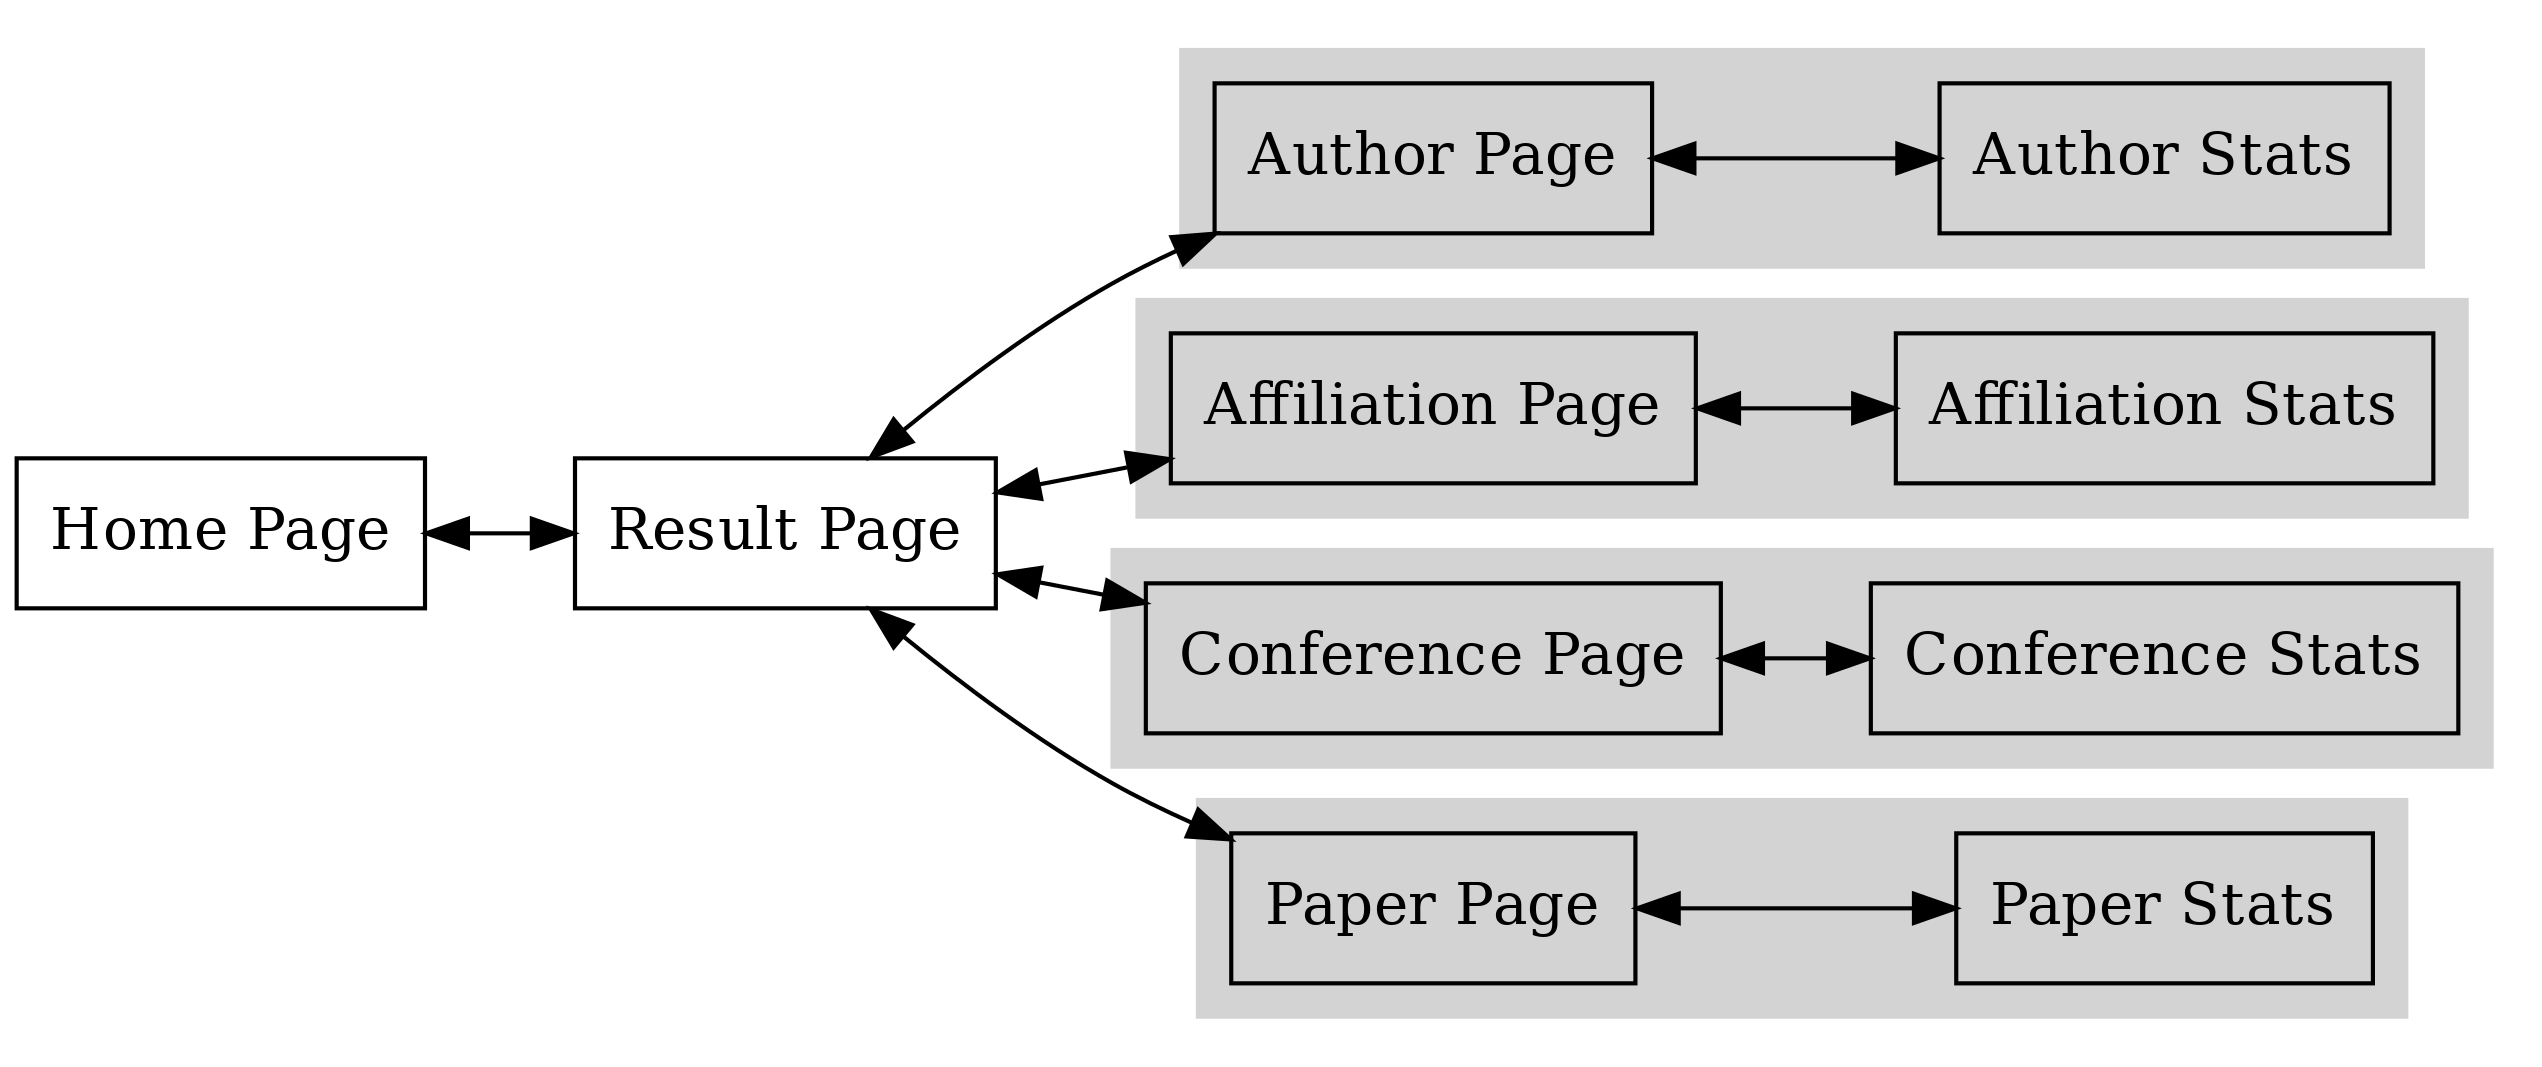
\includegraphics[width=\textwidth]{web_struct.png}
  \caption{The structure of the website}
  \label{fig:web_struct}
\end{figure}
As the chart shows, users will first visit our \textit{Home Page}, input some keywords, and press Enter. The page will redirect to \textit{Result Page}, and after user click one of the links present there, it will jump to the \textit{Information Pages}, which includes \textit{Author Page}, \textit{Affiliation Page}, \textit{Conference Page} and \textit{Paper Page}. From the navigation bar on the top of the \textit{Information Pages}, users can direct to the \textit{Stats Pages} corresponding to the \textit{Information Pages}. All pages can return to the \textit{Result Page} of the most recent query, and the \textit{Home Page}.

\subsubsection{Directory Structure}
In this project we use Code Igniter framework. The framework features MVC design pattern and a bunch of utility and helper funcitons. As a result, we mainly write codes and 
The directory structure of out project is like following:
\paragraph{application}\ 
This directory contains the php scripts that runs on the server and fulfill different jobs. These files mainly fall into three category: controllers, models and views, which follows the MVC design pattern.
\subparagraph{controllers}\ This directory contains the controllers, which is responsible for dealing with the requests and generating responses.
\begin{enumerate}
\item Lab.php\\
  Static Content Controller for all pages. Also provides dynamic content for text queries.
\item Autocomplete.php\\
  Dynamic Content Controller for all input box's auto completion.
\item Label.php\\
  Dynamic Content Controller for label extraction and paper recommendation.
\item Visual.php\\
  Dynamic Content Controller for visualization graphs and charts.
\item Pagin.php\\
  Dynamic Content Controller for pagination bar and corresponding js code.
\end{enumerate}
\subparagraph{models}\ This directory main contains the models which interacts with our database.
\begin{enumerate}
\item Lab\_model.php\\
  Data Provider for all text queries.
\item Visual\_model.php\\
  Data Provider for queries from visualization graphs and charts.
\item Label\_model.php\\
  Data Provider for label extraction and paper recommendation.
\end{enumerate}
\subparagraph{views}\ The directory contains multiple sub-directories: Lab, Multi\_pagin, Shared, Templates.
\begin{enumerate}
\item Lab\\
  This directory contains the "visible" part of the website. It has multiple subdirectories, containing \textbf{page frameworks} and \textbf{page contents} for different kinds of entities, for example authors or affiliations. Besides, it has two individual php files: Home.php, the \textit{Home Page} of the website; Result.frame.php, the framework all-in-one search \textit{Result Page}.
\item Multi\_pagin\\
  This directory contains templates of javascript files used in the pagination system. The controller will process the php files and insert them into the html, and they will be working as ordinary js scripts.
\item Shared\\
  This directory contains the php files for the navigation bar in the top, and some legacy files.
\item Templates\\
  This directory contains the header and the footer. They will be embeded in every web page. \textit{header.php} mainly includes the libraries, and \textit{footer.php} add a banner in the bottom to show the credits.
\end{enumerate}

\paragraph{assets}\
This directory contains the css files and js scripts that will be sent to the client side and processed by the browser.
\subparagraph{css}\
This directory contains the cascading style sheets.
\begin{enumerate}
\item Theme.css\\
  This is the style sheet used by any page you can reach in the website. It defines the the color patterns, fonts and link styles.
\item Search\_selection.css\\
  This is used by the \textit{Home Page}. It defines the color patterns of the search boxes.
\item Visual.css\\
  This is the style sheet used in the visualization part, in particular the force directional graph.
\end{enumerate}
\subparagraph{js}\
This directory contains the javascipt files.
\begin{enumerate}
\item Animation.js\\
  This script adds animations of the search boxes, so that users can collapse and un-collapse them as they like.
\item Authocomplete.js\\
  This script uses jquery to realize ajax search box autocompletion .
\item D3.layout.cloud.js, myplots.js\\
  These scripts defines the behavior of the visulization charts and graphs.
\item sidebar.js\\
  This script animates the side bar.
\item Pagin.js\\
  This script realizes the basic functionality of the pagin system. Itself may not be refernced frequetly as it only supports one pagin bar on one webpage, but it is also the prototype of the dynamic pagin system, which includes the full functionality of the pagin bar and content boxes. 
\end{enumerate}

Overview:
\begin{figure}[H]
  \centering
  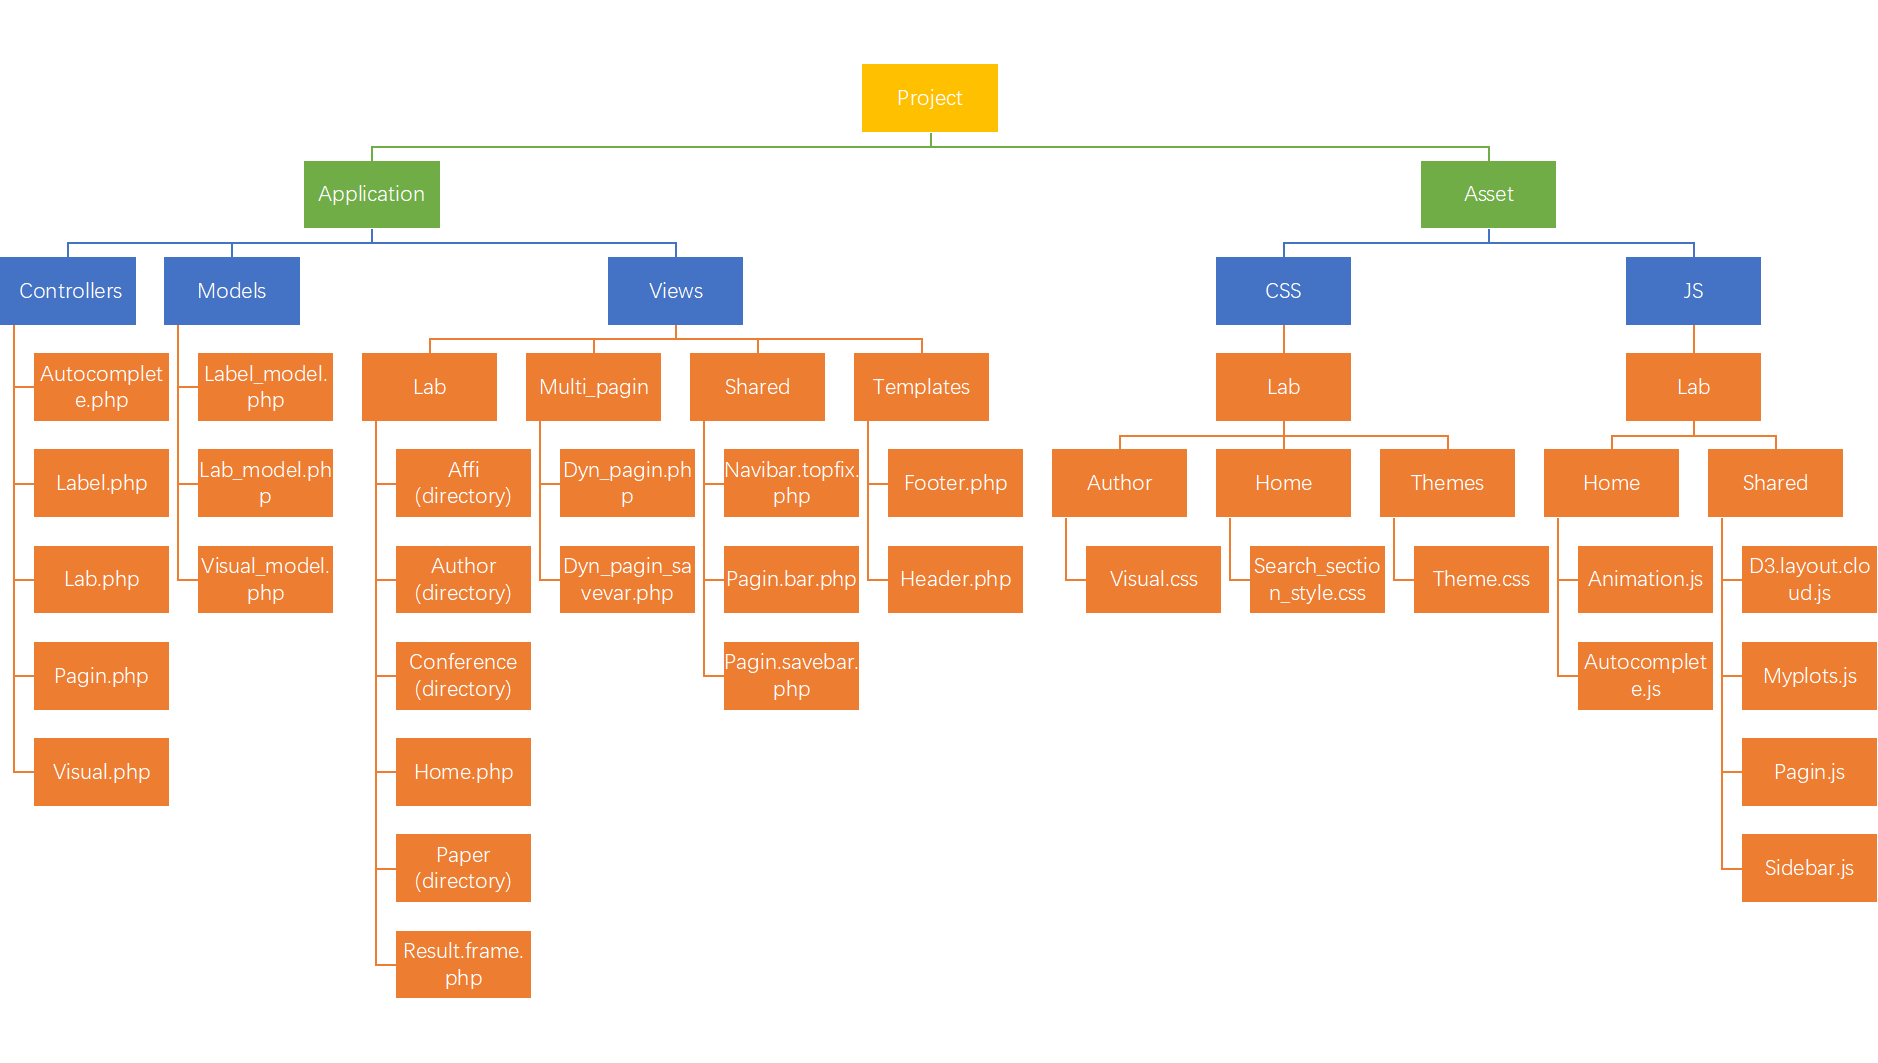
\includegraphics[width=\textwidth]{directory.png}
  \caption{Directory Structure}
  \label{fig:web_struct}
\end{figure}

\subsubsection{Request Process Procedure: \textbf{Page framework} \& \textbf{Page Content}}
The \textit{Result Page}, \textit{Information Pages} and \textit{Stats Pages} all involves many dynamic content loaded by js scripts from client side. To keep things simple, we design a standard and uniform request process procedure, and write some utilitiy functions for it.
The procedure is showed as follows:
\begin{figure}[H]
  \centering
  \caption{Request Process Procedure}
  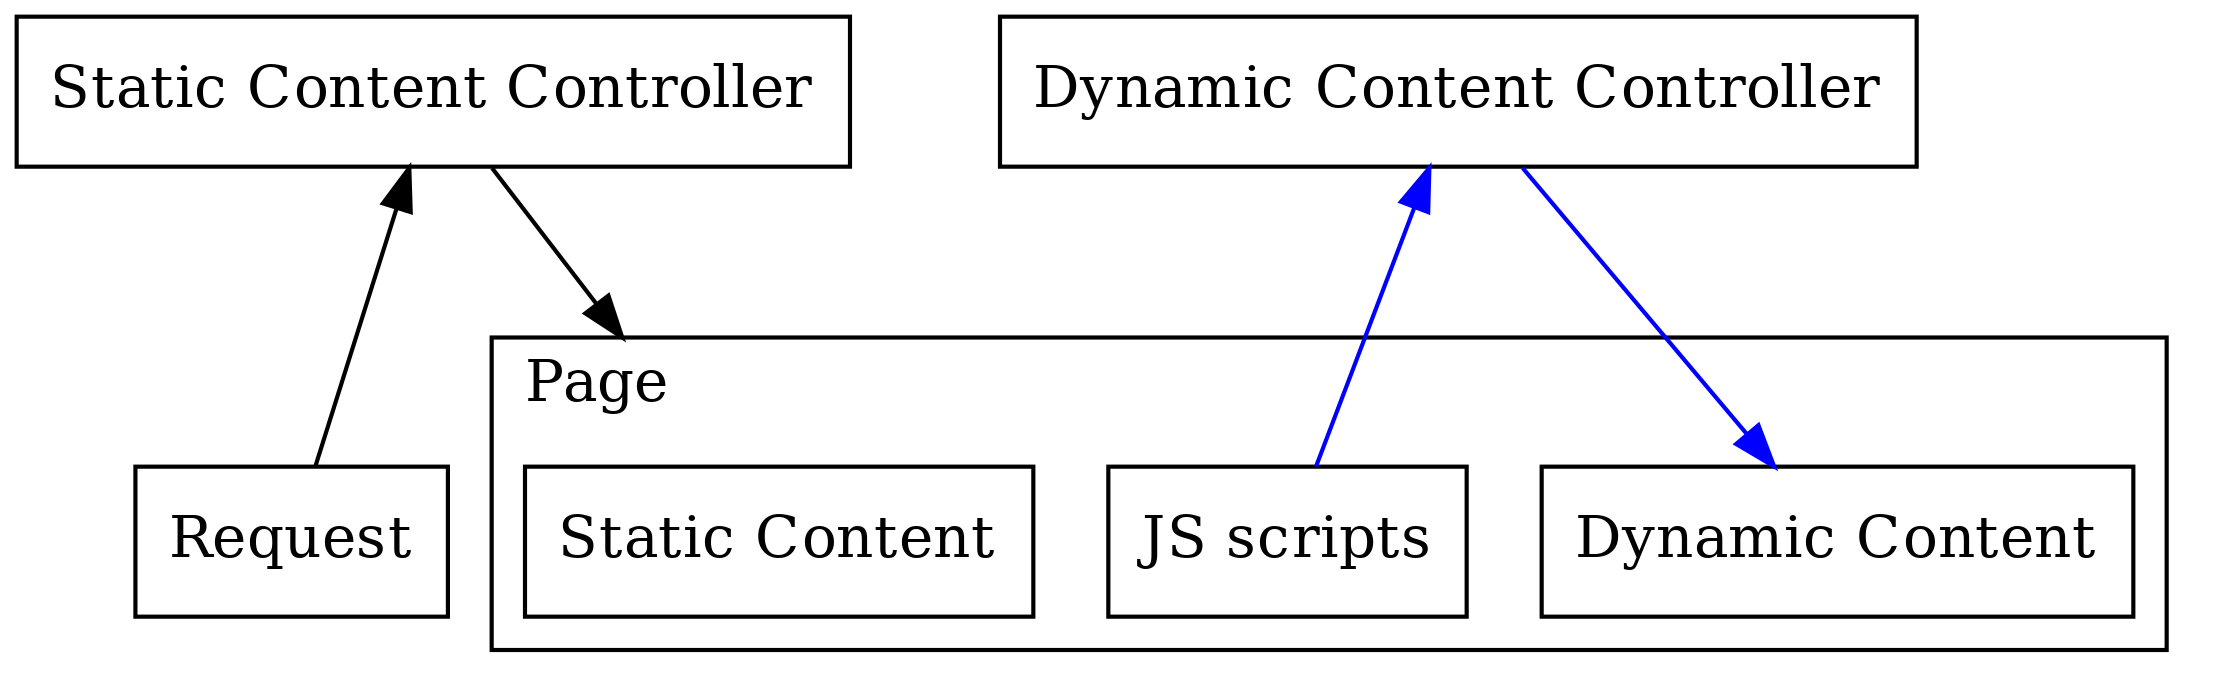
\includegraphics[width=\textwidth]{r_p_p.png}
  \label{fig:r_p_p}
\end{figure}
As the chart shows, whenever the server receives a request, it will first be directed to the static content controller, and the controller will give back the web page containing the static content and the js scripts. We name these things as \textbf{page "framework"s}.
Then the browser interprets the js script, making new requests to the dynamic content controller. After the browser fetches data from the remote, it will present them in the page by ajax, without reloading the whole page. These data or html files are named \textbf{page "content"s}.

\subsection{Project Organization}
%our github cooperation, workload division and building process can be demonstrated here
%zhan
\subsubsection{Workload Division}
\paragraph{Zhan Xinyu} Project structure; Website backend; Utility functions.
\paragraph{Wang Zhongye} Webpage Design; Website frontend, including css and js; Visualization charts.
\paragraph{Xie Yichen} Label Extraction; Page Recommendation. 
\paragraph{Yue Ye} Visualization backend; Slides.
\subsubsection{Collaboration with Git and Github}
To share code and synchronize
\subsubsection{Third party packages and libraries}
\subsubsection{Website Deploy}
\section{Frontend Implementation}
%frontend implementation
%wang
%the interface of back-ends might be mentioned like "The implementation of this functionality will be illustrated in the following sections."
\subsection{Overview}
\subsection{UI Design}
\subsection{Data Visualization}
\section{Functionality Implementation}
%functionality(back-ends) implementation
%except wang
\subsection{Backend Implementation}
In this section we mainly want to talk about how we present the content on server side to the browser running on the client side.

What we have come up with is a set of utility functions, which can be combined and assembled to realize the pagin systemm with which we can process the request and ship the paginated content to the browser.
\paragraph{Pagination Bar Generator}\
\subparagraph{dyn\_pagin.php}\ \\
First of all, we need to write the js code to bind events on the elements. Realizing that there may be more than 1 pagination bar and more than 1 content fetcher in one webpage, we use id to distinguish them so that they can work independently without disturbing each other.

But problem comes: how can we generate the js scripts for different ids? Our solution is to use js script templates.

\textit{dyn\_pagin.php} is a js script template. Before the server send this file to the browser, the php interpreter will process it and fill the \$prefix variable in the variable names. After doing so, it will turn into an html file with a well-functioning js script in it. Then the html file will be sent to the browser with the page framework together.

Following is the first part of the js script template. In this part, a function named <\$prefix>\_pagin\_goto is defined, which launched a request with the local variables stored in the page.
\begin{lstlisting}[language=Javascript]
  function <?php echo $prefix; ?>_pagin_goto() {
    var table_target = <?php echo $prefix; ?>_content_fetch_url + 
    "page=" + <?php echo $prefix; ?>_page +
    "&mode=" + <?php echo $prefix; ?>_field[0] + 
    "&field=" + <?php echo $prefix; ?>_field[1];
    $.get(table_target, function(result){
      $("#" + <?php echo $prefix; ?>_content_handle).html(result);
    });

    var pagin_target = <?php echo $prefix; ?>_pagin_fetch_url + 
    "handle=" + <?php echo $prefix; ?>_pagin_handle +
    "&page=" + <?php echo $prefix; ?>_page +
    "&startpage=" + <?php echo $prefix; ?>_startpage +
    "&endpage=" + <?php echo $prefix; ?>_endpage +
    "&width=" + <?php echo $prefix; ?>_width;
    $.get(pagin_target, function(result) {
      $("#" + <?php echo $prefix; ?>_pagin_handle).html(result);
    });
  }
\end{lstlisting}

Following is the second part of the js script template. In this part, the click events are dynamically binded on the pagination bar elements and realizes the callback functions after the events happen.

The callback function mainly do three things: first extract the target page stored either in the local variables or in the attributes of the pagination bar items, then check the conditions and update the local variables, and finally launched requests to the remote.

\begin{lstlisting}[language=Javascript]
  // bind event: load content when the page is loaded
  $(<?php echo $prefix; ?>_pagin_goto);

  // bind click event: show the content of the first page when the button is pushed down
  $("#" + <?php echo $prefix; ?>_pagin_handle).on(
  'click',
  'a#' + <?php echo $prefix; ?>_pagin_handle + '-begin',
  function() {
    <?php echo $prefix; ?>_page = <?php echo $prefix; ?>_startpage;
    <?php echo $prefix; ?>_pagin_goto();
  });

  //...

  // bind click event: show the content of the given page when the button is pushed down
  $("#" + <?php echo $prefix; ?>_pagin_handle).on(
  'click',
  'a#' + <?php echo $prefix; ?>_pagin_handle + '-item', 
  function() {
    <?php echo $prefix; ?>_page = $(this).attr('pagenum');
    <?php echo $prefix; ?>_pagin_goto();
  });
\end{lstlisting}

\subparagraph{View: dyn\_pagin\_savevar.php}\ \\

Similar to the js script template above, \textit{dyn\_pagin\_savevar.php} is also a script template. It stores the local variables in the webpage.
\begin{lstlisting}[language=Javascript]
  <script>
  var <?php echo $prefix; ?>_page = <?php echo $page; ?>;
  var <?php echo $prefix; ?>_startpage = <?php echo $startpage; ?>;
  var <?php echo $prefix; ?>_endpage = <?php echo $endpage; ?>;
  var <?php echo $prefix; ?>_field = ["<?php echo $field['mode']; ?>", "<?php echo $field["field"]; ?>"];
  var <?php echo $prefix; ?>_width = <?php echo $width; ?>;
  var <?php echo $prefix; ?>_pagin_handle = "<?php echo $pagin_handle; ?>";
  var <?php echo $prefix; ?>_pagin_fetch_url = "<?php echo $pagin_fetch_url; ?>";
  var <?php echo $prefix; ?>_content_handle = "<?php echo $content_handle; ?>";
  var <?php echo $prefix; ?>_content_fetch_url = "<?php echo $content_fetch_url; ?>";
  </script>
\end{lstlisting}

\subparagraph{Controller: Lab.php}\ \\
We have added a utility function to create pagination bars and load the js script templates. It works as an intermediate layer to realize the functionality in a more compact and cleaner way.

This function stores the paginination information(startpage, endpage, current page), style information(bar length, item number), id information(on which element the events will be binded) and route information(the url js will send request to).
\begin{lstlisting}[language=php]
  require "Pagin.php";
  \\...
  private function _makeup_dyn_pagin(
  $prefix, $mode, $field, $total, $nitem, $width,
  $c_hdl, $p_hdl, $c_url, $p_url, &$data)
  {
    $data['prefix'] = $prefix;
    $data['field'] = array(
    "mode" => $mode,
    "field" => $field);
    $data['total_result'] = $total;
    Pagin::_fill_pagenum(1,
    ceil($total / $nitem),
    $data);
    $data['width'] = $width;
    $data['content_handle'] = $c_hdl;
    $data['pagin_handle'] = $p_hdl;
    $data['content_fetch_url'] = $c_url;
    $data['pagin_fetch_url'] = $p_url;

    $this->load->view('multi_pagin/dyn_pagin_savevar.php', $data);
    $this->load->view('multi_pagin/dyn_pagin.php', $data);
  }
\end{lstlisting}

Besides the utility function to help create pagination bars and load script templates, we need more functions to provide the data the users are really interested in. Then we write a set of functions beginning with "view\_", which returns the html files that will be dynamically loaded to the page.

Mainly there are two kinds of these, one is the "view\_<entity>\_table", which is used in the main panel, and the "view\_<entity>\_content", which is used in the sidebar.

Following is an example of authors:
\begin{lstlisting}[language=php]
  public function view_author()
  {
    $data['title'] = "Author Page";
    $data['author_id'] = $this->input->get('author_id');
    $data['author_name'] = $this->Lab_model->get_author($data['author_id'])['AuthorName'];
    $data['item_url'] = get_cookie('query_url');
    
    $this->load->view('templates/header', $data);
    $this->load->view('shared/navibar.topfix.php', $data);
    $this->load->view('lab/author/author.frame.php', $data);

    // dyn pagin loading
    $this->_makeup_dyn_pagin("main", "author_pub", $data['author_id'],
    $this->Lab_model->get_author_pub_total_number($data['author_id']),
    $this->res_per_page, 10,
    "lab-author-main-panel" ,"lab-author-main-pagination",
    base_url()."lab/view_author_content?", 
    base_url()."pagin/pagin_bar?", $data
    );
    $this->_makeup_dyn_pagin("affi", "author_affi", $data['author_id'],
    $this->Lab_model->get_author_affi_total_number($data['author_id']), 5, 5,
    "lab-author-sidebar-af-items", "lab-author-sidebar-af-pagination",
    base_url()."lab/view_author_content?", 
    base_url()."pagin/pagin_bar?", $data
    );
    $this->_makeup_dyn_pagin("conf", "author_conf", $data['author_id'],
    $this->Lab_model->get_author_conf_total_number($data['author_id']), 5, 5,
    "lab-author-sidebar-cf-items", "lab-author-sidebar-cf-pagination",
    base_url()."lab/view_author_content?", 
    base_url()."pagin/pagin_bar?", $data
    );
    $this->_makeup_dyn_pagin("coau", "author_coau", $data['author_id'],
    $this->Lab_model->get_author_coau_total_number($data['author_id']), 5, 5,
    "lab-author-sidebar-ca-items", "lab-author-sidebar-ca-pagination",
    base_url()."lab/view_author_content?", 
    base_url()."pagin/pagin_bar?", $data
    );
    $lbl_count = $this->Label_model->fetch_author_label($data['author_id'],0,0)['num'];
    $this->_makeup_dyn_pagin("labl", "auth_labl", $data['author_id'],
    $lbl_count, 5, 5,
    "lab-author-sidebar-lb-items", "lab-author-sidebar-lb-pagination",
    base_url()."label/view_author_label?", 
    base_url()."pagin/pagin_bar?", $data
    );
    $this->load->view('templates/footer');
  }

  public function view_author_content()
  {
    $mode = $this->input->get('mode');
    $author_id = $this->input->get('field');
    if ($mode == "author_pub") {
      $page = $this->input->get('page');
      if($page===null || $page <= 0)
      $page = 1;
      $pagenum = ($page - 1) * $this->res_per_page;
      
      $retrieve = $this->Lab_model->search_paper_of_author($author_id, $pagenum, $this->res_per_page);
      foreach($retrieve as $index => $content) {
        $retrieve[$index]['ConferenceName'] = 
        $this->Lab_model->get_conference($content['ConferenceID'])['ConferenceName'];
        $retrieve[$index]['AuthorList'] = $this->Lab_model->search_author_of_paper($content['PaperID']);
      }
      
      $data['query_result'] = $retrieve;
      $data['offset'] = $pagenum;
      $data['AuthorListType'] = "link";
      $data['NeedConference'] = true;
      echo $this->load->view('lab/paper/paper.table.php', $data, true);
    } else if ($mode == "author_affi") {
      $page = $this->input->get('page');
      if($page===null || $page <= 0)
      $page = 1;
      $pagenum = ($page - 1) * 5;
      
      $retrieve = $this->Lab_model->search_affi_of_author(
      $author_id, $pagenum, 5);
      $data['query_result'] = $retrieve;
      $data['offset'] = $pagenum;
      echo $this->load->view('lab/affi/affi.content.php', $data, true);
    } else if ($mode == "author_conf") {
      $page = $this->input->get('page');
      if($page===null || $page <= 0)
      $page = 1;
      $pagenum = ($page - 1) * 5;
      
      $retrieve = $this->Lab_model->search_conf_of_author(
      $author_id, $pagenum, 5);
      $data['query_result'] = $retrieve;
      $data['offset'] = $pagenum;
      echo $this->load->view('lab/conference/conference.content.php', $data, true);
    } else if ($mode == "author_coau") {
      $page = $this->input->get('page');
      if($page===null || $page <= 0)
      $page = 1;
      $pagenum = ($page - 1) * 5;
      
      $retrieve = $this->Lab_model->search_coau_of_author(
      $author_id, $pagenum, 5);
      $data['query_result'] = $retrieve;
      $data['offset'] = $pagenum;
      echo $this->load->view('lab/author/coauthor.content.php', $data, true);
    }
  }
\end{lstlisting}

\subparagraph{Views: <entity>.table.php \& <entity>.content.php}\ \\

As metioned above, these php files are part of the "page contents". Still, we use author as an example:

author.table.php (main panel)
\begin{lstlisting}[language=php+html]
  <?php foreach($query_result as $index => $author_item): ?>
  <?php if ($index != 0) { ?>
    <hr>
    <?php } ?>
  <div class="panel-item-title-0 panel-dark-body" >
  <?php echo $offset + $index + 1; ?>.&nbsp&nbsp
  <a href="<?php echo base_url().'lab/view_author?author_id='.$author_item['AuthorID']; ?>" >
  <?php echo ucwords($author_item['AuthorName']); ?>
  </a>
  </div>
  <div class="panel-item-content-0 panel-dark-body" >
  &nbsp&nbsp&nbsp&nbsp&nbsp
  Author ID:&nbsp<?php echo $author_item['AuthorID']; ?>
  &nbsp&nbsp-&nbsp&nbsp
  Paper Published:&nbsp<?php echo $author_item['PaperNum']; ?><br>
  &nbsp&nbsp&nbsp&nbsp&nbsp
  Major Affiliation:&nbsp
  <?php if ($author_item['AffiliationName'] != null) { ?>
    <a href="<?php echo base_url().'lab/view_affi?affi_id='.$author_item['AffiliationID']; ?>" >
    <?php echo ucwords($author_item['AffiliationName']); ?>
    </a>
    <?php }else{ echo "--"; }?>
  </div>

  <?php endforeach; ?>
\end{lstlisting}

author.content.php (side bar)
\begin{lstlisting}[language=php+html]
  <?php foreach($query_result as $index => $author_item): ?>
  <div class="list-group-item" >
  <a href="<?php echo base_url().'lab/view_author?author_id='.$author_item['AuthorID']; ?>"
  ><?php echo ucwords($author_item['AuthorName']); ?></a>
  </div>
  <?php endforeach ?>
\end{lstlisting}

We can see that these are just ordinary html files. As a result, they can be directly inserted to the existing webpage by jquery.

\subsection{Visualization Implementation}
\subsection{Label Extraction}
\subsection{Paper Recommendation}
\section{Future Work}
%future work
%later any one
\section{Conclusion}
%restated what we have accomplished
%later any one

\newpage
\begin{appendices}
  %depends
\end{appendices}
\end{document}
